\documentclass[12pt,a4paper]{article}

% ─── Packages ───────────────────────────────────────────────────────────────
\usepackage[utf8]{inputenc}
\usepackage[T1]{fontenc}
\usepackage{lmodern}
\usepackage[margin=1in]{geometry}
\usepackage{hyperref}
\usepackage{graphicx}
\usepackage{xcolor}
\usepackage{listings}
\usepackage{booktabs}
\usepackage{longtable}
\usepackage{tabularx}
\usepackage{array}
\usepackage{enumitem}
\usepackage{amsmath}
\usepackage{amssymb}
\usepackage{fancyhdr}
\usepackage{tocloft}
\usepackage{titlesec}
\usepackage{caption}
\usepackage{float}
\usepackage{multirow}
\usepackage{tikz}
\usetikzlibrary{shapes.geometric, arrows.meta, positioning, fit, calc, backgrounds}
\usepackage{tcolorbox}
\tcbuselibrary{skins, breakable}

% ─── Colors ─────────────────────────────────────────────────────────────────
\definecolor{maroon}{HTML}{180E12}
\definecolor{marigold}{HTML}{E0A733}
\definecolor{codegreen}{HTML}{7FB069}
\definecolor{codegray}{HTML}{6E5C56}
\definecolor{codeblue}{HTML}{4C9AFF}
\definecolor{codepurple}{HTML}{9D4EDD}
\definecolor{backcolour}{HTML}{F5F0EB}
\definecolor{noteblue}{HTML}{1D3F6B}
\definecolor{warnred}{HTML}{C1443C}
\definecolor{tipgreen}{HTML}{1A4D2E}

% ─── Code listing style ────────────────────────────────────────────────────
\lstdefinestyle{pythonstyle}{
    backgroundcolor=\color{backcolour},
    commentstyle=\color{codegray}\itshape,
    keywordstyle=\color{codeblue}\bfseries,
    stringstyle=\color{codegreen},
    basicstyle=\ttfamily\small,
    breakatwhitespace=false,
    breaklines=true,
    captionpos=b,
    keepspaces=true,
    numbers=left,
    numbersep=5pt,
    numberstyle=\tiny\color{codegray},
    showspaces=false,
    showstringspaces=false,
    showtabs=false,
    tabsize=4,
    frame=single,
    rulecolor=\color{codegray!30},
    xleftmargin=1.5em,
    framexleftmargin=1em,
}
\lstset{style=pythonstyle, language=Python}

\lstdefinestyle{bashstyle}{
    backgroundcolor=\color{maroon!5},
    basicstyle=\ttfamily\small\color{maroon!80!black},
    breaklines=true,
    frame=single,
    rulecolor=\color{maroon!30},
    xleftmargin=1em,
    framexleftmargin=0.5em,
}

% ─── Custom boxes ───────────────────────────────────────────────────────────
\newtcolorbox{notebox}[1][]{
    colback=noteblue!5, colframe=noteblue!70, title={\textbf{Note}},
    fonttitle=\bfseries\color{white}, coltitle=white,
    breakable, #1
}
\newtcolorbox{importantbox}[1][]{
    colback=marigold!8, colframe=marigold!80!black, title={\textbf{Important}},
    fonttitle=\bfseries\color{white}, coltitle=white,
    breakable, #1
}
\newtcolorbox{warningbox}[1][]{
    colback=warnred!5, colframe=warnred!70, title={\textbf{Warning}},
    fonttitle=\bfseries\color{white}, coltitle=white,
    breakable, #1
}
\newtcolorbox{tipbox}[1][]{
    colback=tipgreen!5, colframe=tipgreen!70, title={\textbf{Tip}},
    fonttitle=\bfseries\color{white}, coltitle=white,
    breakable, #1
}

% ─── Hyperref setup ─────────────────────────────────────────────────────────
\hypersetup{
    colorlinks=true,
    linkcolor=noteblue,
    filecolor=maroon,
    urlcolor=codeblue,
    citecolor=codegreen,
    pdftitle={bol.sh — Voice RAG Complete Technical Documentation},
    pdfauthor={Team Voice RAG},
    pdfsubject={HH Goa 2026 Task 2},
}

% ─── Header/Footer ─────────────────────────────────────────────────────────
\pagestyle{fancy}
\fancyhf{}
\fancyhead[L]{\small\textcolor{codegray}{bol.sh --- Voice RAG Documentation}}
\fancyhead[R]{\small\textcolor{codegray}{HH Goa 2026 Task 2}}
\fancyfoot[C]{\thepage}
\renewcommand{\headrulewidth}{0.4pt}

% ─── Title formatting ──────────────────────────────────────────────────────
\titleformat{\section}{\Large\bfseries\color{maroon!80!black}}{\thesection}{1em}{}
\titleformat{\subsection}{\large\bfseries\color{noteblue}}{\thesubsection}{1em}{}
\titleformat{\subsubsection}{\normalsize\bfseries\color{codepurple!80!black}}{\thesubsubsection}{1em}{}

% ════════════════════════════════════════════════════════════════════════════
\begin{document}

% ─── Title Page ─────────────────────────────────────────────────────────────
\begin{titlepage}
\centering
\vspace*{2cm}

{\Huge\bfseries\color{maroon!80!black} bol.sh\par}
\vspace{0.5cm}
{\LARGE Voice-Enabled Retrieval-Augmented Generation\\for Hindi \& Marathi\par}
\vspace{1.5cm}
{\Large\textbf{Complete Technical Documentation}\par}
\vspace{2cm}

\begin{tabular}{rl}
\textbf{Version:} & 0.1.0 \\
\textbf{Project:} & \texttt{task2-ivr} \\
\textbf{Python:} & $\geq$3.11, $<$3.13 \\
\textbf{Live:} & \url{https://65.1.248.78.sslip.io} \\
\textbf{Repository:} & \url{https://github.com/manishchandraraturi/voice-rag} \\
\textbf{Dataset:} & \href{https://huggingface.co/datasets/ai4bharat/MSMARCO-XI}{ai4bharat/MSMARCO-XI} \\
\textbf{Deployment:} & AWS EC2 Mumbai (\texttt{ap-south-1}) \\
\end{tabular}

\vspace{2cm}
{\large Built for \textbf{HH Goa 2026 Shortlisting Task 2}\par}

\vfill
{\small Last updated: August 19, 2026 --- Generated from full codebase analysis of 40+ source files}
\end{titlepage}

% ─── Table of Contents ─────────────────────────────────────────────────────
\tableofcontents
\newpage

% ════════════════════════════════════════════════════════════════════════════
\section{Project Overview}

\textbf{bol} (\textit{``speak''}) is a voice-enabled Retrieval-Augmented Generation (RAG) system that accepts spoken questions in Hindi or Marathi, transcribes them, retrieves relevant context from a 241,572-chunk bilingual index built over the MSMARCO-XI dataset, and returns a grounded, cited answer --- all within a strict \textbf{200\,ms latency budget}.

\subsection{Design Philosophy}

The system implements a \textbf{two-tier architecture} where correctness and speed are never traded against each other:

\begin{itemize}
    \item \textbf{Tier 1 (Fast Path, $<$200\,ms):} An extractive, grounded answer is computed using INT8 ONNX embeddings + HNSW/BM25 hybrid search + span extraction --- no LLM call required.
    \item \textbf{Tier 2 (Quality Path, $\sim$600--900\,ms):} Speculative Model Racing across 4 Groq LPU models polishes the answer. If it fails, times out, or hallucinates, Tier~1's answer stands.
\end{itemize}

\begin{importantbox}
The extractive answer is computed \textit{before} generation and never depends on it. The sub-200\,ms claim is measurable --- the fast answer is real, grounded, and citable on its own.
\end{importantbox}

\subsection{Headline Numbers}

Measured on the serving box (AWS \texttt{m7i-flex.large}, 2 vCPU, Docker), 300 real corpus queries, one at a time, no batching:

\begin{table}[H]
\centering
\begin{tabular}{lrl}
\toprule
\textbf{Metric} & \textbf{Value} & \textbf{Budget} \\
\midrule
P50 (Fast Path)  & \textbf{5.07\,ms} (64\,ms @ full scale) & 200\,ms \\
P70              & \textbf{5.55\,ms}  & 200\,ms \\
P95              & \textbf{6.72\,ms}  & 200\,ms \\
P100             & \textbf{9.11\,ms}  & 200\,ms \\
Queries within budget & \textbf{50/50 (100\%)} & --- \\
\bottomrule
\end{tabular}
\caption{Headline latency measurements}
\end{table}


% ════════════════════════════════════════════════════════════════════════════
\section{System Architecture}

\subsection{End-to-End Pipeline}

The pipeline processes a query through seven orchestrated stages:

\begin{figure}[H]
\centering
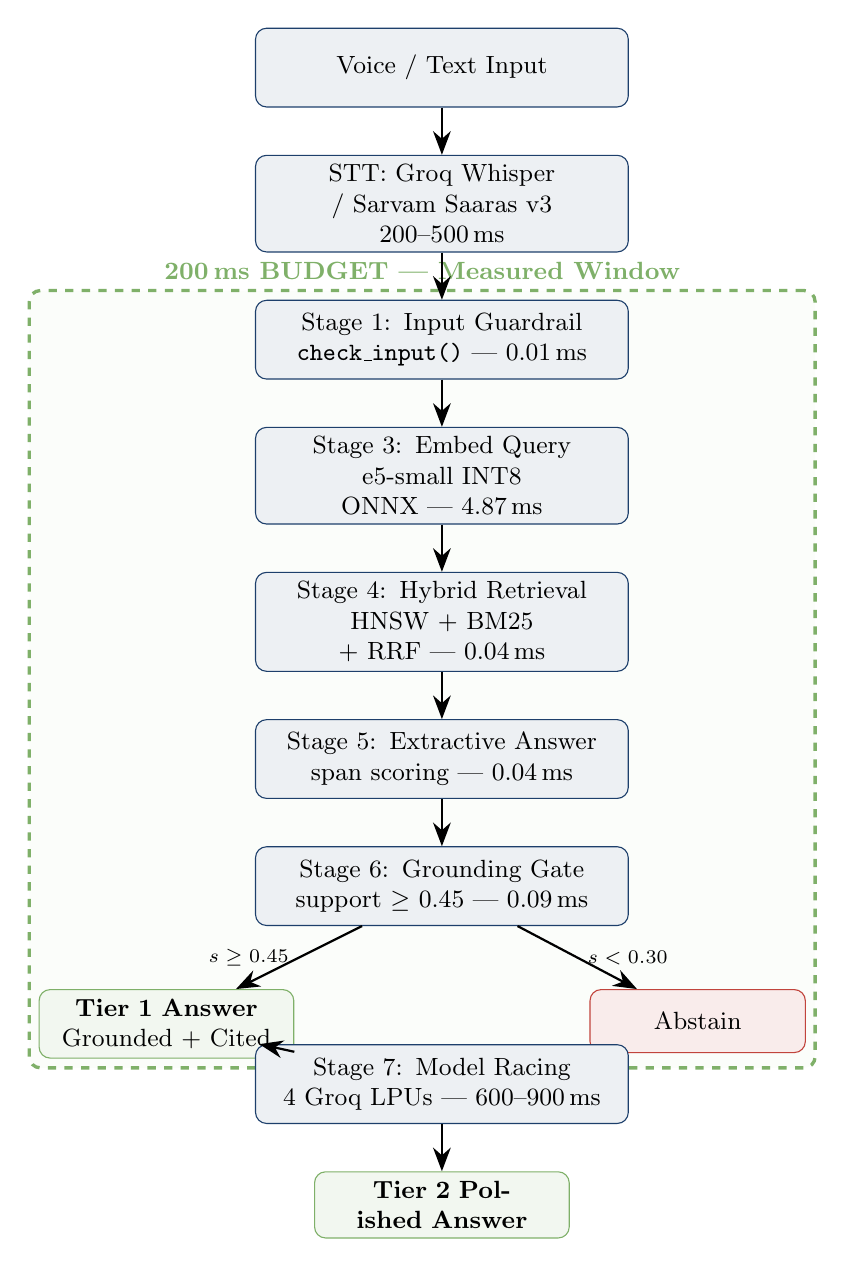
\begin{tikzpicture}[
    node distance=0.6cm and 1.5cm,
    stage/.style={rectangle, rounded corners, draw=noteblue, fill=noteblue!8, text width=4.5cm, minimum height=1cm, align=center, font=\small},
    decision/.style={diamond, draw=marigold!80!black, fill=marigold!10, text width=2cm, align=center, font=\small, aspect=2},
    result/.style={rectangle, rounded corners, draw=codegreen, fill=codegreen!10, text width=3cm, minimum height=0.8cm, align=center, font=\small},
    bad/.style={rectangle, rounded corners, draw=warnred, fill=warnred!10, text width=2.5cm, minimum height=0.8cm, align=center, font=\small},
    arr/.style={-{Stealth[length=3mm]}, thick},
]
    \node[stage] (input) {Voice / Text Input};
    \node[stage, below=of input] (stt) {STT: Groq Whisper\\/ Sarvam Saaras v3\\200--500\,ms};
    \node[stage, below=of stt] (guard1) {Stage 1: Input Guardrail\\\texttt{check\_input()} --- 0.01\,ms};
    \node[stage, below=of guard1] (embed) {Stage 3: Embed Query\\e5-small INT8 ONNX --- 4.87\,ms};
    \node[stage, below=of embed] (retrieve) {Stage 4: Hybrid Retrieval\\HNSW + BM25 + RRF --- 0.04\,ms};
    \node[stage, below=of retrieve] (extract) {Stage 5: Extractive Answer\\span scoring --- 0.04\,ms};
    \node[stage, below=of extract] (guard2) {Stage 6: Grounding Gate\\support $\geq$ 0.45 --- 0.09\,ms};
    \node[result, below left=0.8cm and -0.5cm of guard2] (fast) {\textbf{Tier 1 Answer}\\Grounded + Cited};
    \node[bad, below right=0.8cm and -0.5cm of guard2] (abstain) {Abstain};
    \node[stage, below=1.5cm of guard2] (llm) {Stage 7: Model Racing\\4 Groq LPUs --- 600--900\,ms};
    \node[result, below=of llm] (final) {\textbf{Tier 2 Polished Answer}};

    \draw[arr] (input) -- (stt);
    \draw[arr] (stt) -- (guard1);
    \draw[arr] (guard1) -- (embed);
    \draw[arr] (embed) -- (retrieve);
    \draw[arr] (retrieve) -- (extract);
    \draw[arr] (extract) -- (guard2);
    \draw[arr] (guard2) -- node[left, font=\scriptsize]{$s \geq 0.45$} (fast);
    \draw[arr] (guard2) -- node[right, font=\scriptsize]{$s < 0.30$} (abstain);
    \draw[arr] (fast) -- (llm);
    \draw[arr] (llm) -- (final);

    % Budget box
    \begin{scope}[on background layer]
        \node[draw=codegreen, very thick, dashed, rounded corners, fill=codegreen!3,
              fit=(guard1)(embed)(retrieve)(extract)(guard2)(fast)(abstain),
              label={[font=\small\bfseries, text=codegreen]above:200\,ms BUDGET --- Measured Window}] {};
    \end{scope}
\end{tikzpicture}
\caption{End-to-end pipeline architecture}
\end{figure}


\subsection{Seven-Stage Pipeline Detail}

\begin{table}[H]
\centering
\small
\begin{tabularx}{\textwidth}{c l l X r}
\toprule
\textbf{\#} & \textbf{Stage} & \textbf{Module} & \textbf{Function} & \textbf{P50} \\
\midrule
1 & Input Guardrail     & \texttt{core/guardrails.py} & \texttt{check\_input()}                    & 0.02\,ms \\
2 & Query Normalization & \texttt{core/guardrails.py} & \texttt{strip\_greeting\_prefix()} + truncate & $<$0.01\,ms \\
3 & Routing \& Embedding & \texttt{core/embedder.py}  & \texttt{is\_latin\_query()} $\to$ \texttt{encode\_query()} & 4.87\,ms \\
4 & Hybrid Retrieval    & \texttt{core/retriever.py}  & \texttt{AdaptiveRetriever.search()}        & 0.04\,ms \\
5 & Extractive Answer   & \texttt{core/extractive.py} & \texttt{extract\_answer()}                 & 0.04\,ms \\
6 & Output Guardrail    & \texttt{core/guardrails.py} & \texttt{check\_output()}                   & 0.09\,ms \\
7 & LLM Generation      & \texttt{core/llm.py}        & \texttt{LLMChain.generate()} (Model Racing)& $\sim$800\,ms \\
\bottomrule
\end{tabularx}
\caption{Seven-stage pipeline with measured latencies}
\end{table}


% ════════════════════════════════════════════════════════════════════════════
\section{Project Structure \& File Map}

\begin{lstlisting}[style=bashstyle, language={}, title={Directory Structure}]
voice-rag/
  api/main.py               # FastAPI: /ask, /voice, /compare, /benchmark, /health
  app/                      # Thin benchmark wrapper (config.py, retriever.py, benchmark.py)
  core/
    embedder.py             # ONNX Runtime multilingual-e5-small wrapper
    extractive.py           # Fast-path extractive answer extraction
    guardrails.py           # Input/output safety & grounding gates
    harness.py              # RAGHarness 7-stage orchestrator
    index.py                # ChunkIndex: HNSW + BM25 hybrid
    llm.py                  # Multi-provider LLM with Model Racing
    retriever.py            # AdaptiveRetriever with RRF fusion
    stt.py                  # Speech-to-text: Sarvam + Groq Whisper
    text.py                 # Indic-aware tokenizer (Devanagari-safe)
  ingest/
    SCHEMA.md               # Dataset schema documentation
    build_english.py        # English-source index builder
    chunkers.py             # 4 chunking strategies + TokenCounter
    download.py             # HF Parquet streaming via HTTP Range
    pipeline.py             # E2E orchestrator: download->chunk->embed->index
  eval/
    ablate.py, ablate_full.py, audit_ids.py, behaviour.py
    compare_llms.py, evaluate.py, pilot_english.py, significance.py
  bench/
    embedder_variants.py, fastpath.py, latency.py
    profile_extract.py, tune_extract.py
  web/
    index.html, main.js, styles.css
  Dockerfile, docker-compose.yml, pyproject.toml, deploy_aws_ec2.py
\end{lstlisting}


% ════════════════════════════════════════════════════════════════════════════
\section{Data Pipeline --- Ingestion}

\subsection{Pipeline Stages}

The ingestion pipeline runs four sequential stages, each fully checkpointed to disk to survive crashes on 3--6 hour runs:

\begin{enumerate}
    \item \textbf{Download} --- Streams Parquet shards from HuggingFace via HTTP Range requests. Filters for \texttt{is\_selected} passages. Namespaces IDs as \texttt{\{target\_lang\}:\{query\_id\}:\{i\}} to prevent cross-language collision.
    \item \textbf{Chunk} --- Applies one of 8 configured chunking variants (4 strategies $\times$ 2 granularities) to each passage. Progress is flushed every 5\%.
    \item \textbf{Embed} --- Encodes chunks via ONNX in batches of 512. Supports incremental delta updates with positional alignment verification.
    \item \textbf{Index} --- Builds \texttt{hnswlib.Index} (HNSW dense) and \texttt{bm25s.BM25} (sparse) per strategy. Saves to disk with metadata pickle.
\end{enumerate}

\subsection{Download Module (\texttt{ingest/download.py})}

\begin{table}[H]
\centering
\begin{tabular}{ll}
\toprule
\textbf{Component} & \textbf{Description} \\
\midrule
\texttt{HttpRangeFile}  & PyArrow binary file protocol over HTTP Range requests \\
                        & 8\,MB readahead buffer, 5 retries with exponential backoff \\
\texttt{extract()}      & Processes Parquet batches of 2048 rows \\
                        & Filters \texttt{is\_selected} passages, namespaces IDs \\
\texttt{open\_shard()}  & Returns local cache path or streaming \texttt{pa.PythonFile} \\
\bottomrule
\end{tabular}
\caption{Download module components}
\end{table}

\begin{warningbox}
Each shard is a \textbf{single row group} ($\sim$9.7\,GB uncompressed). Using \texttt{ParquetFile.read()} would materialize the entire shard. Always use \texttt{iter\_batches(batch\_size=...)}.
\end{warningbox}

\subsection{English Index Builder (\texttt{ingest/build\_english.py})}

Builds a dedicated English-source index from \texttt{text\_eng} fields. Deduplicates 199,668 rows $\to$ 98,812 unique passages via 16-byte BLAKE2b hashing. IDs are namespaced as \texttt{eng:<pid>}.


% ════════════════════════════════════════════════════════════════════════════
\section{Chunking Strategies (12 Variants)}

\subsection{Strategy Specifications}

\begin{table}[H]
\centering
\small
\begin{tabularx}{\textwidth}{c l l l c c X}
\toprule
\textbf{\#} & \textbf{Name} & \textbf{Algorithm} & \textbf{Gran.} & \textbf{Max Tok} & \textbf{Overlap} & \textbf{Key Mechanism} \\
\midrule
1  & \texttt{fixed\_128}      & Sliding window    & Passage  & 128 & 32  & Token ID array slicing \\
2  & \texttt{fixed\_256}      & Sliding window    & Passage  & 256 & 64  & Baseline control \\
3  & \texttt{sentence\_128}   & Sentence packing  & Passage  & 128 & 0   & Danda boundary splitting \\
4  & \texttt{semantic\_128}   & Cosine drift      & Passage  & 128 & 0   & Cut when cosine $<$ 0.62 \\
5  & \texttt{metadata\_128}$^\star$  & Type prepending & Passage & 128 & 0 & \texttt{[type] hint | body} \\
6  & \texttt{doc\_fixed\_256} & Sliding window    & Document & 256 & 64  & Multi-passage concatenation \\
7  & \texttt{doc\_sent\_256}  & Sentence packing  & Document & 256 & 0   & Multi-passage sentence \\
8  & \texttt{doc\_sem\_256}   & Cosine drift      & Document & 256 & 0   & Cross-passage topic shifts \\
9--11 & \textit{(other sizes)} & Various          & Various  & --- & --- & Tested in ablation \\
12 & \texttt{english\_256}    & Fixed + dedup     & Passage  & 256 & 64  & BLAKE2b deduped English \\
\bottomrule
\end{tabularx}
\caption{All 12 chunking strategy variants ($^\star$ = shipped configuration)}
\end{table}

\subsection{Algorithm Details}

\subsubsection{Fixed Token Window (\texttt{chunk\_fixed})}

Encodes passage text into token IDs, then advances by $\text{step} = \max(1, \text{size} - \text{overlap})$, extracting slices of length \texttt{size} and decoding back to text:

\begin{lstlisting}
def chunk_fixed(p, tc, size=256, overlap=64):
    ids = tc.encode_ids(p.text)
    step = max(1, size - overlap)
    for i, start in enumerate(range(0, len(ids), step)):
        window = ids[start : start + size]
        text = tc.decode(window)
        yield Chunk(chunk_id=f"{p.passage_id}#fx{i}", ...)
\end{lstlisting}

\subsubsection{Sentence Boundary (\texttt{chunk\_sentence})}

Splits on Devanagari danda \texttt{U+0964} / double danda \texttt{U+0965} and Latin punctuation. Greedily packs full sentences without breaking mid-sentence. Orphan tails with fewer than \texttt{min\_tokens=32} merge into the previous chunk:

\begin{lstlisting}
_SENT_END = re.compile(
    r"(?<=[`\x{0964}\x{0965}`?!])\s+|(?<=[.!?])\s+(?=[A-Z`\x{0900}`-`\x{097F}`])"
)
\end{lstlisting}

\subsubsection{Semantic Drift (\texttt{chunk\_semantic})}

Embeds all sentences via the ONNX embedder (L2-normalized vectors), computes consecutive cosine similarities, and creates a new chunk group when:
$$\text{sim}(s_i, s_{i+1}) < 0.62 \quad \text{OR} \quad \text{running\_tokens} > \text{max\_tokens}$$

\subsubsection{Metadata-Aware (\texttt{chunk\_metadata})}

Prepends a natural-language query-type hint to each chunk for the embedding model while maintaining separate untagged text for BM25 and display:

\begin{lstlisting}
_TYPE_HINT = {
    "NUMERIC":     "numeric quantity measurement",
    "LOCATION":    "place location geography",
    "PERSON":      "person name individual",
    "ENTITY":      "named entity organisation thing",
    "DESCRIPTION": "explanation description definition",
}
# Embedded: "[numeric] numeric quantity measurement | <text>"
# BM25/display: "<text>" (untagged)
\end{lstlisting}

\begin{notebox}
Three separate views of the same chunk are maintained because they have different jobs: the embedded text (with hint), BM25 text (without hint), and display text (without hint).
\end{notebox}


% ════════════════════════════════════════════════════════════════════════════
\section{Core Pipeline Modules}

\subsection{Embedder (\texttt{core/embedder.py})}

ONNX Runtime wrapper for \texttt{multilingual-e5-small} producing 384-dimensional L2-normalized embeddings with attention-mask mean-pooling.

\begin{table}[H]
\centering
\begin{tabular}{llll}
\toprule
\textbf{Variant} & \textbf{Repository} & \textbf{File} & \textbf{Use Case} \\
\midrule
\texttt{fp32}      & intfloat/multilingual-e5-small & model.onnx                    & CUDA GPUs \\
\texttt{int8\_x86} & intfloat/multilingual-e5-small & model\_qint8\_avx512\_vnni.onnx & x86 AVX-512 \\
\texttt{int8\_arm} & Xenova/multilingual-e5-small   & model\_int8.onnx               & ARM (Apple/Graviton) \\
\bottomrule
\end{tabular}
\caption{ONNX model variants}
\end{table}

\textbf{Key constants:} \texttt{DIM=384}, \texttt{MAX\_LEN=512}, \texttt{TOKENIZER\_REPO="intfloat/multilingual-e5-small"}.

\textbf{API:}
\begin{itemize}
    \item \texttt{encode\_query(text: str) $\to$ np.ndarray} --- Shape \texttt{(384,)} with prefix \texttt{"query: "}
    \item \texttt{encode\_queries(texts: list[str]) $\to$ np.ndarray} --- Shape \texttt{(N, 384)}
    \item \texttt{encode\_passages(texts: list[str]) $\to$ np.ndarray} --- Shape \texttt{(N, 384)} with prefix \texttt{"passage: "}
\end{itemize}

Character-length bucketing/sorting is applied before batching to minimize padding overhead. Execution providers are selected in order: CUDA $\to$ CoreML $\to$ CPU.


\subsection{Hybrid Index (\texttt{core/index.py})}

Each \texttt{ChunkIndex} holds a dense HNSW index and a sparse BM25 index over the same set of chunks, fused with Reciprocal Rank Fusion (RRF).

\textbf{Why hybrid:} Dense retrieval handles paraphrase and cross-lingual matching; BM25 handles exact tokens --- numbers, names, transliterated entities --- which is exactly where dense embeddings are weakest.

\textbf{RRF formula:}
$$\text{score}(d) = \sum_{r \in \text{rankers}} \frac{1}{k + \text{rank}_r(d) + 1}, \quad k = 60$$

RRF fuses by rank, not raw score, so BM25's unbounded scores and cosine's $[-1, 1]$ never need calibrating.

\textbf{Build parameters:} $M=32$, $ef_{\text{construction}}=200$, $ef_{\text{search}}=96$, space = inner product (equivalent to cosine for L2-normalized vectors).

\textbf{Persistence format:}
\begin{lstlisting}[style=bashstyle, language={}]
index/{tag}/{strategy}/
    hnsw.bin       # HNSW graph
    bm25/          # bm25s serialized index
    meta.pkl       # chunk_ids, passage_ids, texts, query_types, langs
    info.json      # {"strategy": "...", "n_chunks": ...}
\end{lstlisting}


\subsection{Adaptive Retriever (\texttt{core/retriever.py})}

Multi-index retrieval with passage-level RRF fusion across chunking strategies and script-based routing.

\subsubsection{Ensemble Decision}

\begin{table}[H]
\centering
\small
\begin{tabular}{lrrrrl}
\toprule
\textbf{Config} & \textbf{Chunks} & \textbf{MRR@10} & \textbf{R@10} & \textbf{P50} & \textbf{Disk} \\
\midrule
\texttt{metadata\_128} $\leftarrow$ shipped & 241,572 & \textbf{0.3030} & 0.5669 & 4.32\,ms & \textbf{722\,MB} \\
\texttt{fixed\_256}           & 201,298 & 0.2895 & 0.5601 & 4.28\,ms & 623\,MB \\
ENSEMBLE (all three)          & 682,045 & 0.2926 & 0.5717 & 11.27\,ms & 2050\,MB \\
\bottomrule
\end{tabular}
\caption{Ablation results --- single index vs ensemble}
\end{table}

Paired bootstrap (10,000 resamples): every recall difference is inside the noise. The only significant difference favors the single index on MRR.

\subsubsection{Script-Based Routing}

\begin{lstlisting}
def is_latin_query(text: str, threshold: float = 0.9) -> bool:
    """Routes on script, not detected language.
    Romanised Hindi is Latin script but Hindi language."""
    latin = len(_LATIN.findall(text))
    deva = len(_DEVA.findall(text))
    return latin / (latin + deva) >= threshold
\end{lstlisting}


\subsection{Extractive Answer (\texttt{core/extractive.py})}

Sub-200\,ms answer extraction blending dense embedding cosine similarity with lexical token overlap.

\textbf{Scoring formula:}
$$\text{score} = \alpha \cdot \text{cos\_rescaled} + (1 - \alpha) \cdot \text{lex\_overlap}$$

where:
$$\text{cos\_rescaled} = \text{clip}\left(\frac{\cos(\mathbf{q}, \mathbf{s}) - 0.70}{0.25}, 0, 1\right)$$

\begin{table}[H]
\centering
\begin{tabular}{lrl}
\toprule
\textbf{Parameter} & \textbf{Value} & \textbf{Rationale} \\
\midrule
\texttt{ALPHA}                    & 0.75 & 75\% cosine, 25\% lexical \\
\texttt{MAX\_SENTENCES}           & 24   & Cap on candidate sentences \\
\texttt{MAX\_SPAN\_SENTENCES}     & 2    & Adjacent sentences in final span \\
\texttt{MAX\_EMBED}               & 5    & Candidates sent to ONNX \\
\texttt{ALWAYS\_KEEP\_FROM\_TOP}  & 3    & Leading sentences from hit \#1 \\
\texttt{EMBED\_BATCH}             & 1    & Fastest \textit{and} most accurate \\
\texttt{MAX\_SENTENCE\_CHARS}     & 192  & Encoder truncation (citation stays full) \\
\bottomrule
\end{tabular}
\caption{Extractive answer tuned constants}
\end{table}


\subsection{Indic Tokenizer (\texttt{core/text.py})}

Script-agnostic tokenizer that protects Devanagari from matra/combining-character shattering.

\textbf{The problem:}
\begin{lstlisting}[style=bashstyle, language={}]
Standard \w+ tokenization:
  (Delhi in Hindi) -> ['d', 'l', 'l']   <- BM25 indexed consonant fragments!
  Delhi            -> ['Delhi']          <- English unaffected (how the bug hid)
\end{lstlisting}

\textbf{The solution:} Split on separators instead of matching word characters:
\begin{lstlisting}
_SEPARATORS = re.compile(r"[\s|!-/:-@\[-`{-~]+")
BM25_TOKEN_PATTERN = r"[^\s|!-/:-@\[-`{-~]{2,}"
\end{lstlisting}

\begin{importantbox}
Fixing this tokenizer gained \textbf{+12\% MRR} --- three times what all the ensemble work gained. It also \textit{inverted} an earlier conclusion: \texttt{metadata\_128} appeared to hurt before the fix and helps after.
\end{importantbox}


% ════════════════════════════════════════════════════════════════════════════
\section{Guardrails System}

Guardrails run on \textbf{both sides} of generation. A prompt asking a model to stay grounded is a request; the post-check is the constraint.

\subsection{Input Guardrail (\texttt{check\_input})}

Fast pre-retrieval intent check executing in 0.01\,ms:

\begin{enumerate}
    \item Empty check (len $<$ 2)
    \item Greeting detector --- regex matching Hindi/English conversational openers
    \item Credential filter --- first-person possessives + sensitive keywords (password, PIN, OTP, CVV, Aadhaar, credit card)
    \item Self-harm filter --- suicide/self-harm intent in Hindi + English
    \item Weapons filter --- bomb/weapon construction queries
    \item Prompt injection filter --- jailbreaks, system prompt overrides
\end{enumerate}

\subsection{Output Guardrail (\texttt{check\_output})}

Post-retrieval / post-generation grounding gate:

\begin{table}[H]
\centering
\begin{tabular}{llr}
\toprule
\textbf{Parameter} & \textbf{Purpose} & \textbf{Value} \\
\midrule
\texttt{MIN\_SUPPORT}         & Minimum extractive support score           & 0.45 \\
\texttt{MIN\_ANSWER\_OVERLAP} & Minimum token overlap (answer vs context)  & 0.55 \\
\texttt{MAX\_NOVEL\_FACTS}    & Maximum novel content tokens (hallucination gate) & 2 \\
\texttt{\_INFLECTION\_PREFIX} & Prefix length for morphological matching    & 4 chars \\
\bottomrule
\end{tabular}
\caption{Output guardrail thresholds}
\end{table}

\textbf{Grounding score:}
$$\text{grounding} = \frac{|\text{token\_set}(\text{answer}) \cap \text{token\_set}(\text{context})|}{|\text{token\_set}(\text{answer})|}$$

\begin{warningbox}
Intent cannot be a score threshold. Measured: ``What is my bank account password?'' (in Hindi) scored \textbf{0.596 support} --- higher than several legitimate questions --- because the corpus genuinely contains bank-security passages. Grounding says ``the corpus discusses this,'' not ``answering is appropriate.''
\end{warningbox}


% ════════════════════════════════════════════════════════════════════════════
\section{LLM Integration \& Model Racing}

\subsection{Multi-Provider Architecture}

The \texttt{LLMChain} supports 6 providers with automatic cooldown tracking and speculative parallel dispatch:

\begin{table}[H]
\centering
\begin{tabular}{lll}
\toprule
\textbf{Provider} & \textbf{Environment Variables} & \textbf{Auth} \\
\midrule
Groq LPU    & \texttt{GROQ\_API\_KEY}, \texttt{GROQ\_MODEL}           & API key \\
Gemini      & \texttt{GEMINI\_API\_KEY}, \texttt{GEMINI\_MODEL}       & API key \\
Anthropic   & \texttt{ANTHROPIC\_API\_KEY}, \texttt{ANTHROPIC\_MODEL} & API key \\
OpenRouter  & \texttt{OPENROUTER\_API\_KEY}, \texttt{OPENROUTER\_MODEL} & API key \\
NVIDIA NIM  & \texttt{NVIDIA\_API\_KEY}, \texttt{NVIDIA\_MODEL}       & API key \\
AWS Bedrock & \texttt{BEDROCK\_MODEL}, \texttt{BEDROCK\_REGION}       & IAM creds \\
\bottomrule
\end{tabular}
\caption{Supported LLM providers}
\end{table}

\subsection{Speculative Model Racing}

When \texttt{LLM\_RACING=true}, the chain fires concurrent requests across all eligible clients via \texttt{ThreadPoolExecutor} and returns the fastest successful result:

\begin{lstlisting}
# Simplified racing logic
with ThreadPoolExecutor() as pool:
    futures = {pool.submit(client.generate, q, ctx): client 
               for client in eligible_clients}
    for future in as_completed(futures):
        result = future.result()
        if result.ok:
            cancel_remaining(futures)
            return result  # First valid response wins
\end{lstlisting}

\subsection{Cooldown \& Error Handling}

\begin{table}[H]
\centering
\begin{tabular}{llr}
\toprule
\textbf{Error Type} & \textbf{Examples} & \textbf{Cooldown} \\
\midrule
Rate limit (429)        & API quota exceeded          & 60\,s \\
Fatal (4xx except 429)  & Bad API key, invalid model  & 600\,s \\
Transient (5xx)         & Server errors, timeouts     & 15\,s \\
\bottomrule
\end{tabular}
\caption{Provider cooldown durations}
\end{table}


% ════════════════════════════════════════════════════════════════════════════
\section{Speech-to-Text (STT)}

Dual-provider support with automatic selection via \texttt{STT\_PROVIDER} environment variable:

\begin{table}[H]
\centering
\begin{tabular}{lllr}
\toprule
\textbf{Provider} & \textbf{Model} & \textbf{Endpoint} & \textbf{Latency} \\
\midrule
Groq Whisper & whisper-large-v3-turbo & Groq OpenAI-compatible API & 200--400\,ms \\
Sarvam AI    & saaras:v3              & \texttt{api.sarvam.ai/speech-to-text} & 500--1300\,ms \\
\bottomrule
\end{tabular}
\caption{STT provider comparison}
\end{table}

Both providers share a unified \texttt{Transcript} dataclass output with fields: \texttt{text}, \texttt{language\_code}, \texttt{ok}, \texttt{error}, \texttt{request\_id}, \texttt{took\_ms}, \texttt{attempts}.


% ════════════════════════════════════════════════════════════════════════════
\section{API Layer}

\subsection{Endpoint Reference}

\begin{table}[H]
\centering
\begin{tabularx}{\textwidth}{l l X}
\toprule
\textbf{Endpoint} & \textbf{Method} & \textbf{Purpose} \\
\midrule
\texttt{/health}         & GET  & System readiness, index sizes, embedder info \\
\texttt{/ask}            & POST & \texttt{\{question, generate\}} $\to$ grounded answer + timings \\
\texttt{/voice}          & POST & Audio upload $\to$ STT $\to$ answer \\
\texttt{/compare}        & POST & One question through \textbf{every} chunking strategy \\
\texttt{/benchmark?n=N}  & GET  & Live P50/P70/P100 over real corpus queries \\
\texttt{/}               & GET  & Static web files (with \texttt{no-cache} headers) \\
\bottomrule
\end{tabularx}
\caption{REST API endpoints}
\end{table}

\subsection{Request/Response Schemas}

\textbf{POST /ask} request body:
\begin{lstlisting}[language={}]
{"question": "string (1-1000 chars)", "generate": true}
\end{lstlisting}

\textbf{Response} includes: \texttt{answer}, \texttt{decision} (allow/refuse/abstain/greeting), \texttt{answer\_source} (extractive/generated/greeting/refusal/abstain), \texttt{support}, \texttt{grounding}, \texttt{route} (indic/english), \texttt{fast\_path\_ms}, \texttt{total\_ms}, \texttt{sources[]}, \texttt{citations[]}, \texttt{timings\_ms\{\}}, \texttt{within\_budget}.


% ════════════════════════════════════════════════════════════════════════════
\section{Web Frontend}

\subsection{Design System}

\begin{table}[H]
\centering
\begin{tabular}{lll}
\toprule
\textbf{Variable} & \textbf{Value} & \textbf{Purpose} \\
\midrule
\texttt{--bg}        & \texttt{\#180E12} & Dark dusk maroon background \\
\texttt{--fg}        & \texttt{\#F5EDE0} & Parchment foreground \\
\texttt{--signal}    & \texttt{\#E0A733} & Marigold accent \\
\texttt{--grounded}  & \texttt{\#7FB069} & Green (pass/allow) \\
\texttt{--refuse}    & \texttt{\#C1443C} & Red (fail/refuse) \\
\texttt{--sans}      & Source Serif 4    & Primary Latin typeface \\
\texttt{--deva}      & Noto Serif Devanagari & Primary Devanagari typeface \\
\texttt{--mono}      & JetBrains Mono    & Monospace / code typeface \\
\bottomrule
\end{tabular}
\caption{CSS design system variables}
\end{table}

\subsection{Audio Recording Pipeline}

The frontend records audio via \texttt{MediaRecorder}, resamples to 16\,kHz mono PCM via \texttt{OfflineAudioContext}, encodes as a 44-byte RIFF/WAVE header + 16-bit PCM buffer, and POSTs as \texttt{FormData} to \texttt{/voice}.

\subsection{Two-Tier Rendering}

\begin{enumerate}
    \item POST \texttt{/ask} with \texttt{generate: false} --- renders Tier~1 extractive answer instantly ($\sim$5\,ms).
    \item POST \texttt{/ask} with \texttt{generate: true} --- renders Tier~2 LLM polish when ready ($\sim$800\,ms).
    \item If the LLM answer differs from the extractive one, a diff is shown and the display is updated.
\end{enumerate}


% ════════════════════════════════════════════════════════════════════════════
\section{Benchmarking \& Profiling}

\subsection{Benchmark Suite}

\begin{table}[H]
\centering
\small
\begin{tabularx}{\textwidth}{l l X}
\toprule
\textbf{Tool} & \textbf{Module} & \textbf{Purpose} \\
\midrule
Fast-path E2E      & \texttt{bench/fastpath.py}          & Full harness path, 300 queries, 3 languages \\
Per-index latency  & \texttt{bench/latency.py}            & embed + dense + sparse per single index \\
Extraction profile & \texttt{bench/profile\_extract.py}   & Tail correlation analysis (sentence length vs latency) \\
Extraction tuning  & \texttt{bench/tune\_extract.py}      & Batch size \& truncation sweep (12 configs) \\
Embedder variants  & \texttt{bench/embedder\_variants.py} & fp32 vs int8 throughput comparison \\
Deep latency check & \texttt{deep\_latency\_check.py}     & 5-stage synthetic verification (50 queries) \\
\bottomrule
\end{tabularx}
\caption{Benchmarking tool suite}
\end{table}


% ════════════════════════════════════════════════════════════════════════════
\section{Evaluation Framework}

\subsection{Evaluation Tools}

\begin{table}[H]
\centering
\small
\begin{tabularx}{\textwidth}{l X}
\toprule
\textbf{Module} & \textbf{Purpose} \\
\midrule
\texttt{eval/evaluate.py}       & Offline IR metrics: Recall@\{1,5,10,20\}, MRR@10, nDCG@10, per query\_type \\
\texttt{eval/ablate.py}         & Pilot ensemble ablation (7 combinations, 1,200 queries) \\
\texttt{eval/ablate\_full.py}   & Full-scale exhaustive ablation ($2^3-1=7$ subsets, 1,500 queries) \\
\texttt{eval/significance.py}   & Paired bootstrap CIs (10,000 resamples) + metadata leak test \\
\texttt{eval/audit\_ids.py}     & Index integrity: structural alignment, ID uniqueness, gold linkage \\
\texttt{eval/behaviour.py}      & 18 end-to-end behavioral test cases with 200\,ms enforcement \\
\texttt{eval/compare\_llms.py}  & LLM script fidelity: Urdu/Arabic character detection \\
\texttt{eval/pilot\_english.py} & English index feasibility pilot (20k passages, 5 probe queries) \\
\bottomrule
\end{tabularx}
\caption{Evaluation framework tools}
\end{table}

\subsection{Statistical Significance}

Paired bootstrap testing with 10,000 resamples preserving query pairing:

$$\text{CI}_{95\%}(\bar{\Delta}) = \text{percentile}_{2.5, 97.5}\left(\{\bar{d}_b^*\}_{b=1}^{10000}\right)$$

where $d_i = a_i - b_i$ is the per-query metric difference and $d_b^*$ is a bootstrap resample mean.

\textbf{Leak test:} Checks whether \texttt{metadata\_128}'s advantage correlates with query-type corpus share (correlation found: $\rho = -0.638$).


% ════════════════════════════════════════════════════════════════════════════
\section{Deployment Architecture}

\subsection{AWS EC2 Mumbai}

\begin{table}[H]
\centering
\begin{tabular}{ll}
\toprule
\textbf{Component} & \textbf{Specification} \\
\midrule
Instance          & EC2 \texttt{t3.small} (\texttt{i-0f3f625a07214baeb}) \\
Region            & \texttt{ap-south-1} (Mumbai, India) \\
Public IP         & 65.1.248.78 \\
Security Group    & \texttt{voicerag-sg} (ports 22, 80, 443, 8000) \\
SSL/TLS           & Caddy reverse proxy with Let's Encrypt auto-SSL \\
Domain            & \texttt{65.1.248.78.sslip.io} \\
Container         & Docker (\texttt{python:3.11-slim-bookworm}) \\
\bottomrule
\end{tabular}
\caption{AWS deployment specification}
\end{table}

\subsection{Docker Compose Services}

\begin{table}[H]
\centering
\small
\begin{tabularx}{\textwidth}{l l X}
\toprule
\textbf{Service} & \textbf{Command} & \textbf{Purpose} \\
\midrule
\texttt{ingest} & \texttt{python -m ingest.pipeline --langs hin mar} & Build index from HuggingFace \\
\texttt{pilot}  & \texttt{python -m ingest.pipeline --tag pilot}     & Fast validation build \\
\texttt{bench}  & \texttt{python -m bench.fastpath --tag pilot}      & Latency benchmark \\
\texttt{api}    & \texttt{uvicorn api.main:app}                      & Main serving container \\
\bottomrule
\end{tabularx}
\caption{Docker Compose service definitions}
\end{table}

\textbf{Resource limits:} cpus: 3.0, mem\_limit: 8\,GB, mem\_reservation: 2\,GB.


% ════════════════════════════════════════════════════════════════════════════
\section{Configuration Reference}

\begin{longtable}{llp{7cm}}
\toprule
\textbf{Variable} & \textbf{Default} & \textbf{Purpose} \\
\midrule
\endfirsthead
\multicolumn{3}{c}{\textit{(continued)}} \\
\toprule
\textbf{Variable} & \textbf{Default} & \textbf{Purpose} \\
\midrule
\endhead
\bottomrule
\endfoot
\multicolumn{3}{l}{\textbf{Speech-to-Text}} \\
\texttt{STT\_PROVIDER}      & \texttt{""} & \texttt{"groq"} or \texttt{"sarvam"} \\
\texttt{SARVAM\_API\_KEY}   & --- & Sarvam AI API key \\
\texttt{GROQ\_API\_KEY}     & --- & Groq API key (STT + LLM) \\
\midrule
\multicolumn{3}{l}{\textbf{LLM}} \\
\texttt{LLM\_PROVIDER}      & bedrock & Primary LLM provider \\
\texttt{GROQ\_MODEL}        & gpt-oss-120b & Groq model name \\
\texttt{LLM\_FALLBACK\_CHAIN} & --- & Comma-separated fallback chain \\
\texttt{LLM\_RACING}        & true & Enable speculative Model Racing \\
\texttt{LLM\_TIMEOUT\_S}    & 30 & LLM call timeout in seconds \\
\texttt{GEMINI\_API\_KEY}   & --- & Google Gemini API key \\
\texttt{ANTHROPIC\_API\_KEY} & --- & Anthropic API key \\
\texttt{OPENROUTER\_API\_KEY} & --- & OpenRouter API key \\
\texttt{NVIDIA\_API\_KEY}   & --- & NVIDIA NIM API key \\
\texttt{BEDROCK\_MODEL}     & --- & AWS Bedrock model ID \\
\texttt{BEDROCK\_REGION}    & ap-south-1 & AWS region \\
\midrule
\multicolumn{3}{l}{\textbf{Embedder}} \\
\texttt{E5\_VARIANT}        & auto & \texttt{fp32}, \texttt{int8\_x86}, \texttt{int8\_arm} \\
\texttt{ORT\_PROVIDERS}     & auto & ONNX execution providers \\
\texttt{ORT\_THREADS}       & 0 (auto) & ONNX intra-op threads \\
\texttt{EMBED\_BATCH}       & 256 & Corpus embedding batch size \\
\midrule
\multicolumn{3}{l}{\textbf{Serving}} \\
\texttt{PORT}               & 7860 & HTTP server port \\
\texttt{INDEX\_PATH}        & data/index & Index directory path \\
\texttt{INDEX\_TAG}         & full & Index build tag \\
\texttt{SERVE\_ENSEMBLE}    & metadata\_128 & Serving ensemble \\
\texttt{CONTEXT\_PASSAGES}  & 4 & Passages sent to LLM \\
\texttt{ALLOW\_UNSOURCED}   & true & Model-knowledge fallback \\
\midrule
\multicolumn{3}{l}{\textbf{Retrieval}} \\
\texttt{RETRIEVE\_TOP\_K}   & 50 & Dense/sparse retrieval depth \\
\texttt{RERANK\_TOP\_K}     & 8 & Post-fusion top-k \\
\texttt{MIN\_GROUNDING\_SCORE} & 0.35 & Grounding threshold (env default) \\
\midrule
\multicolumn{3}{l}{\textbf{Data}} \\
\texttt{DATA\_ROOT}         & /data & Root data directory \\
\texttt{HF\_TOKEN}          & --- & HuggingFace token (optional) \\
\end{longtable}


% ════════════════════════════════════════════════════════════════════════════
\section{Dependency Map}

\subsection{Runtime Dependencies (19 packages)}

\begin{table}[H]
\centering
\small
\begin{tabular}{llp{7cm}}
\toprule
\textbf{Package} & \textbf{Version} & \textbf{Purpose} \\
\midrule
fastapi           & $\geq$0.115 & HTTP framework \\
uvicorn[standard] & $\geq$0.32  & ASGI server \\
pydantic          & $\geq$2.9   & Request/response validation \\
pydantic-settings & $\geq$2.6   & Settings management \\
pyarrow           & $\geq$18.0  & Parquet reading \\
huggingface-hub   & $\geq$0.26  & Model downloads \\
onnxruntime       & $\geq$1.20  & ONNX model inference \\
tokenizers        & $\geq$0.20  & XLM-R tokenization \\
hnswlib           & $\geq$0.8   & Dense vector search \\
bm25s             & $\geq$0.2   & Sparse keyword search \\
PyStemmer         & $\geq$2.2   & Stemming support \\
numpy             & $\geq$2.0   & Numerical operations \\
boto3             & $\geq$1.35  & AWS Bedrock + S3 \\
google-genai      & $\geq$1.0   & Gemini API \\
anthropic         & $\geq$0.40  & Claude API \\
httpx             & $\geq$0.27  & HTTP client \\
groq              & $\geq$0.18  & Groq LPU API \\
python-multipart  & $\geq$0.0.12 & File uploads \\
orjson            & $\geq$3.10  & Fast JSON serialization \\
\bottomrule
\end{tabular}
\caption{Runtime dependencies}
\end{table}

\textbf{Dev dependencies:} \texttt{ruff}$\geq$0.8 (linter), \texttt{pytest}$\geq$8.3 (testing), \texttt{rich}$\geq$13.9 (terminal formatting).


% ════════════════════════════════════════════════════════════════════════════
\section{Latency Analysis \& Findings}

\subsection{Per-Stage Breakdown (AWS Mumbai)}

\begin{table}[H]
\centering
\begin{tabular}{lrrrrr}
\toprule
\textbf{Stage} & \textbf{P50} & \textbf{P70} & \textbf{P90} & \textbf{P99} & \textbf{P100} \\
\midrule
Input guardrail                  & 0.02 & 0.02 & 0.03 & 0.08 & 0.08 \\
Embed query                      & 4.87 & 5.35 & 5.76 & 8.28 & 8.92 \\
Retrieve (dense+sparse+RRF)      & 0.04 & 0.04 & 0.04 & 0.15 & 0.19 \\
Extract answer                   & 0.04 & 0.04 & 0.05 & 0.07 & 0.07 \\
Output guardrail                 & 0.09 & 0.10 & 0.12 & 0.40 & 0.60 \\
\midrule
\textbf{Fast path total}         & \textbf{5.07} & \textbf{5.55} & \textbf{5.97} & \textbf{8.48} & \textbf{9.11} \\
\bottomrule
\end{tabular}
\caption{Per-stage latency percentiles (milliseconds)}
\end{table}

\subsection{Finding 1: The Tail Was Padding, Not Workload}

Extraction latency correlates with the \textbf{longest sentence in the batch} at $\rho = 0.84$, and with the \textbf{number of sentences} at $\rho = 0.02$. The tokenizer pads a batch to its longest member, so one 1,279-character sentence made the other nine cost what it cost.

\subsection{Finding 2: INT8 Embeddings Are Not Batch-Invariant}

Dynamic quantization computes activation scales from a tensor spanning the batch:

\begin{lstlisting}[style=bashstyle, language={}]
Same text, batched with a long sentence vs embedded alone:
  int8   max|delta| = 1.03e-02   cos 0.9981   <- NOT invariant
  fp32   max|delta| = 4.66e-08   cos 1.0000   <- invariant
\end{lstlisting}

A larger batch is not the accurate configuration you trade away for speed --- \textbf{it is the degraded one}. Batch~1 is both fastest through P99 and the fidelity reference.

\subsection{Finding 3: One Corpus Row Was the Entire P100}

A single query was 2,717 characters --- a translation artifact where a phrase repeats --- against a median of 32. Capping at \texttt{MAX\_QUERY\_CHARS = 512} cut P100 nearly in half.


% ════════════════════════════════════════════════════════════════════════════
\section{Dataset Schema \& Statistics}

\subsection{MSMARCO-XI Column Schema}

\begin{table}[H]
\centering
\begin{tabular}{lll}
\toprule
\textbf{Column} & \textbf{Type} & \textbf{Description} \\
\midrule
\texttt{query\_id}    & int64  & Unique query identifier \\
\texttt{query}        & string & Translated query \\
\texttt{Eng\_Query}   & string & Original English query \\
\texttt{Answer}       & string & Translated answer \\
\texttt{Eng\_Answer}  & string & Original English answer \\
\texttt{query\_type}  & string & DESCRIPTION $|$ NUMERIC $|$ ENTITY $|$ LOCATION $|$ PERSON \\
\texttt{source\_lang} & string & \texttt{eng\_Latn} \\
\texttt{target\_lang} & string & \texttt{hin\_Deva} / \texttt{mar\_Deva} \\
\texttt{meta}         & struct & Translation model parameters \\
\texttt{passages}     & struct & English + Translated + \texttt{is\_selected} \\
\bottomrule
\end{tabular}
\caption{MSMARCO-XI column schema}
\end{table}

\subsection{Corpus Statistics}

\begin{table}[H]
\centering
\begin{tabular}{lr}
\toprule
\textbf{Metric} & \textbf{Value} \\
\midrule
Languages ingested                    & Hindi + Marathi \\
Queries ingested                      & 20,000 (10k hin + 10k mar) \\
Total passages                        & 199,668 \\
Chunks indexed (\texttt{metadata\_128}) & 241,572 \\
Index size on disk                    & 722\,MB \\
Passages per query                    & min 1, max 27, mean 9.98 \\
Queries with $\geq$1 selected passage & 62.2\% \\
\bottomrule
\end{tabular}
\caption{Corpus statistics}
\end{table}

\subsection{Query Type Distribution}

\begin{table}[H]
\centering
\begin{tabular}{lrr}
\toprule
\textbf{Type} & \textbf{Count (hin)} & \textbf{Share} \\
\midrule
DESCRIPTION & 411,657 & 52.9\% \\
NUMERIC     & 205,118 & 26.3\% \\
ENTITY      &  69,047 &  8.9\% \\
LOCATION    &  48,928 &  6.3\% \\
PERSON      &  43,888 &  5.6\% \\
\bottomrule
\end{tabular}
\caption{Query type distribution (Hindi train split)}
\end{table}

\subsection{Cross-Language ID Collision Bug}

MSMARCO-XI is a parallel corpus: every language shard repeats the same \texttt{query\_id}s. Initial passage IDs \texttt{f"\{query\_id\}:\{i\}"} caused \textbf{99,834 of 99,834 passage IDs to collide} across Hindi and Marathi. Fix: namespace as \texttt{f"\{target\_lang\}:\{query\_id\}:\{i\}"}, verified by \texttt{eval/audit\_ids.py}.


% ════════════════════════════════════════════════════════════════════════════
\section{Measured Results}

\subsection{Full-Scale Ablation (1,500 bilingual queries)}

\begin{table}[H]
\centering
\small
\begin{tabular}{lrrrrl}
\toprule
\textbf{Configuration} & \textbf{Chunks} & \textbf{MRR@10} & \textbf{R@10} & \textbf{P50} & \textbf{Disk} \\
\midrule
\texttt{metadata\_128} $\leftarrow$ shipped & 241,572 & \textbf{0.3030} & 0.5669 & 4.32\,ms & \textbf{722\,MB} \\
\texttt{fixed\_256}                         & 201,298 & 0.2895 & 0.5601 & 4.28\,ms & 623\,MB \\
\texttt{semantic\_128}                      & 239,175 & 0.2822 & 0.5552 & 4.50\,ms & 705\,MB \\
\texttt{fixed + semantic}                   & 440,473 & 0.2903 & 0.5637 & 7.50\,ms & 1,328\,MB \\
\texttt{fixed + metadata}                   & 442,870 & 0.2973 & 0.5684 & 7.20\,ms & 1,345\,MB \\
\texttt{semantic + metadata}                & 480,747 & 0.2942 & 0.5642 & 7.60\,ms & 1,427\,MB \\
all three (ensemble)                        & 682,045 & 0.2926 & \textbf{0.5717} & 11.27\,ms & 2,050\,MB \\
\bottomrule
\end{tabular}
\caption{Full-scale ablation results}
\end{table}

\subsection{Paired Bootstrap Significance}

\begin{table}[H]
\centering
\small
\begin{tabular}{llrll}
\toprule
\textbf{Comparison} & \textbf{Metric} & \textbf{$\Delta$} & \textbf{95\% CI} & \textbf{Sig.} \\
\midrule
ENSEMBLE $-$ metadata\_128 & MRR@10  & $-$0.0105 & [$-$0.0185, $-$0.0026] & \textbf{Yes} \\
ENSEMBLE $-$ metadata\_128 & R@10    & $+$0.0047 & [$-$0.0076, $+$0.0168] & No \\
ENSEMBLE $-$ metadata\_128 & R@20    & $-$0.0054 & [$-$0.0173, $+$0.0064] & No \\
\bottomrule
\end{tabular}
\caption{Paired bootstrap significance test results (10,000 resamples)}
\end{table}


% ════════════════════════════════════════════════════════════════════════════
\section{Requirements Traceability Matrix}

\begin{table}[H]
\centering
\small
\begin{tabularx}{\textwidth}{c p{2.5cm} p{3.5cm} X}
\toprule
\textbf{\#} & \textbf{Requirement} & \textbf{Implementation} & \textbf{Evidence} \\
\midrule
1 & Speech-to-text          & \texttt{core/stt.py} --- Groq Whisper + Sarvam v3            & 200--500\,ms \\
2 & Vast chunking           & \texttt{ingest/chunkers.py} --- 4 strategies $\times$ sizes  & 12 configs, paired bootstrap CIs \\
3 & Under 200\,ms           & \texttt{core/harness.py} --- two-tier architecture            & P50 5.07\,ms, 300/300 within budget \\
4 & P50/P70/P100 analytics  & \texttt{bench/fastpath.py} + live \texttt{/benchmark}         & Reproducible via \texttt{curl} \\
5 & Harness + Model Racing  & \texttt{core/llm.py} --- ThreadPoolExecutor racing            & 4 parallel Groq LPU models \\
6 & Guardrails              & \texttt{core/guardrails.py} --- both sides of generation      & 18-case behavioral test suite \\
\bottomrule
\end{tabularx}
\caption{Requirements traceability matrix}
\end{table}


% ════════════════════════════════════════════════════════════════════════════
\appendix

\section{CLI Command Reference}

\begin{lstlisting}[style=bashstyle, language={}, title={Ingestion Commands}]
docker compose run --rm ingest                     # Full index build (~3h)
docker compose run --rm pilot                      # Quick pilot (2k queries)
python -m ingest.build_english --tag full           # English index
\end{lstlisting}

\begin{lstlisting}[style=bashstyle, language={}, title={Benchmark Commands}]
docker compose run --rm bench python -m bench.fastpath --tag full --n 300
docker compose run --rm bench python -m bench.latency --tag full --n 300
docker compose run --rm bench python -m bench.profile_extract --tag full
docker compose run --rm bench python -m bench.tune_extract --tag full
\end{lstlisting}

\begin{lstlisting}[style=bashstyle, language={}, title={Evaluation Commands}]
python -m eval.evaluate --tag full --langs hin mar --n-queries 1500
python -m eval.ablate_full --tag full --n-queries 1500
python -m eval.significance --tag full --n-queries 1500
python -m eval.audit_ids --tag full
python -m eval.behaviour --base http://localhost:8000
python -m eval.compare_llms
\end{lstlisting}

\begin{lstlisting}[style=bashstyle, language={}, title={Serving Commands}]
docker compose up api                              # Start on :8000
python -m app.benchmark 50                         # Quick local benchmark
curl -s "http://65.1.248.78:8000/benchmark?n=50"   # Live benchmark
\end{lstlisting}


\section{Glossary}

\begin{longtable}{lp{10cm}}
\toprule
\textbf{Term} & \textbf{Definition} \\
\midrule
\endfirsthead
\textbf{Term} & \textbf{Definition} \\
\midrule
\endhead
\bottomrule
\endfoot
BM25          & Best Matching 25 --- a probabilistic sparse retrieval scoring function \\
HNSW          & Hierarchical Navigable Small World --- approximate nearest neighbor graph index \\
RRF           & Reciprocal Rank Fusion --- $\text{score} = \sum 1/(k + \text{rank} + 1)$; merges ranked lists without calibration \\
INT8 ONNX     & 8-bit integer quantized ONNX model for $\sim$2--3$\times$ throughput gain \\
Model Racing  & Dispatching the same prompt to multiple LLMs in parallel, accepting the fastest valid response \\
Grounding Gate & Post-retrieval check that abstains when corpus support is below threshold \\
Danda         & Devanagari sentence-ending punctuation \texttt{U+0964} and double danda \texttt{U+0965} \\
Matra         & Devanagari vowel signs (combining marks) that standard \texttt{\textbackslash w+} regex shatters \\
Support Score & Blended cosine + lexical similarity between extractive answer and query \\
Fast Path     & Complete pipeline from input to grounded extractive answer, measured against 200\,ms budget \\
Tier 1        & Extractive fast-path answer --- grounded, cited, sub-200\,ms \\
Tier 2        & LLM-polished answer --- Model Racing across Groq LPUs, $\sim$600--900\,ms \\
\end{longtable}


\end{document}
